%!TEX root = ../dissertation.tex
\section{Small RNA Therapeutics and Pharmacology} \label{sec:discussion:therapy}
\subsection{Interactions Between Small Molecule Drugs and Small RNAs}
While we know a lot about the transcriptional effects of approved small molecule drugs, and likewise have learned much about the workings of miRNAs in regulating the transcriptome, knowledge about the intersection between small molecule drug effects and miRNAs (and other small RNAs) \emph{in vivo} is still lacking. There have been reports of miRNA regulation conveying drug resistance in single instances (mainly in cancer);\cite{Ma2010} for example, the deletion of the genomic locus containing the miR-125b gene led to an increased susceptibility of breast cancer patients to anthracylines.\cite{Climent2007} There have been attempts at comprehensively assessing the potential interaction spaces between drug- and miRNA-effects,\cite{Meng2016, Xie2019} however, these are limited to indirect comparison of the transcript spectra of drugs and miRNAs compared (»drug \textbf{A} influences expression of gene \textbf{B}, which is also influenced by miRNA \textbf{C}, so there may be interaction«), and text mining. Both examples are relatively crude estimations of possible interactions, feature a low resolution, and disregard tissue-specific effects and transcription factor interactions, both of which are elementary in the effects of most approved transcriptionally relevant drugs.\cite{Clayton2018}

While a majority of drug-miRNA interactions is still in the dark, it is feasible that miRNAs not only convey drug resistance, but may also play a part in the known effects of approved small molecule drugs, particularly those with known transcriptional effects, such as \acfp{gc}. There have been single reports of miRNA perturbations upon treatment with antipsychotics such as Halo"-per"-i"-dol, Clozapine, and Chlorpromazine, but those reports are seldom and remain descriptive.\cite{Gardiner2014} Clayton and colleagues have recently reviewed the role of miRNAs in \ac{gc} action.\cite{Clayton2018} They found that miRNAs modulate the biogenesis of GCs in the adrenal glands as well as cell responses to GCs. At least part of the effects of GCs in cell function, proliferation, and survival are conveyed via their regulation of miRNA expression. The GC receptor is regulated by miRNAs, such that a repression of the receptor by up-regulated miRNAs conveyed treatment resistance in leukaemias and asthma. In leukocytes, miR-155 down-regulation is an important aspect of GC-mediated suppression of inflammation; dexamethasone-mediated suppression of the response to \acf{lps} inhibited the up-regulation of miR-155 in primary macrophages, macrophage cell lines, spleen and liver cells of mice, and T cells of sepsis patients.\cite{Clayton2018} In our hands, dexamethasone prevented the up-regulation of the top six stroke-perturbed \acfp{trf} in murine RAW 264.7 macrophages \emph{in vitro}.\cite{Winek2020}

GCs also inhibit the expression of miR-101, which leads to impaired \acf{mapk} activation and subsequent suppression of inflammation. Resistance to GC-induced apoptosis in multiple myeloma has been associated with elevations of miR-221/222 and miR-125b. Paradoxically, GCs themselves increase the expression of miR-125b, which may constitute a negative feedback mechanism, partly via suppression of p53.\cite{Murray2013} Notably, members of the mir-10/199 families (see Section \ref{sec:cellculture:mir-go}) are closely intertwined with regulation of GC function. In addition to the aforementioned effects of miR-125b on GC action, miR-125a and miR-10b regulate GC synthesis via interaction with CYP11B1 and CYP11B2 (11-Deoxycorticosterone $\to$ Corticosterone $\to$ Aldosterone; 11-Deoxycortisol $\to$ Cortisol), whereas miR-199a is up-regulated by GC treatment of osteoblasts and conveys WNT pathway suppression, and miR-199a levels were found to be reduced in patients with Cushing's disease. Clayton \emph{et al.}\cite{Clayton2018} also identify major hurdles in the development of therapeutic strategies paying respect to miRNA involvement, which are congruent with my own assessment. The first refers to the complex biological role of small RNAs and the challenges it presents to bioinformatics: 

\begin{quote}
»How are functional interactions to be predicted with confidence, and how are subtle effects of individual miRNAs to be experimentally validated without the danger of confirmation bias? How are miRNA-mediated effects on biological processes to be identified and understood when they involve many-to-many rather than one-to-one interactions?«
\end{quote}

The second refers to the challenge in translating the biological knowledge so gained into effective treatment:

\begin{quote}
»Even where good therapeutic targets can be clearly identified, it remains to be seen whether a mimic or antagonist of a single miRNA species will be sufficient to exert therapeutic effects. If targeting more than one miRNA proves necessary, this will create additional barriers to development, in part because of the problem of predicting and mitigating off-target effects.«
\end{quote}

These questions imply that mimicking or antagonism of an endogenous miRNA (or multiple) may not be the most logical way of pursuing small RNA therapeutic applications, which will be addressed in the following section (\ref{sec:discussion:smrna-therapy}).

\subsection{Small RNAs as Pharmacological Agents} \label{sec:discussion:smrna-therapy}
Application of small oligonucleotides in therapy of human diseases is in the early stages of development. Theoretically, antisense oligonucleotides can, via their instrumentalisation of endogenous RNA interference machinery, silence virtually any gene in the human body, including non-coding genes. Thus, presuming an appropriate design strategy, synthetic oligonucleotides possess a broader spectrum than traditional small molecule drugs. Because of their chemical nature, i.e., high molecular weight and poly-ionised backbone, oligonucleotides cannot cross biological membranes via passive diffusion and therefore have to be delivered using pharmaceutical technology, most commonly, lipid nanoparticles (Figure \ref{fig:lipid}).\cite{Akhtar2007, Whitehead2009} Additionally, to circumvent recognition by the host defence system, e.g. by \acp{tlr}, the bases composing the oligonucleotide are often chemically modified. Common modifications include the 2'-O-methyl sugar modification, which prevents TLR7-mediated response, bridging between two sugar molecule carbon atoms (creating so-called »locked nucleic acids«), which fix the nucleotides in a specific steric position, and hybridisation to molecules such as cholesterol or polyethylene glycol, which can convey steric hindrance and even organ targeting properties.\cite{Whitehead2009}

\begin{figure}
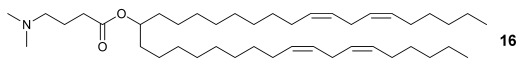
\includegraphics[width=\textwidth]{figures/mfig004}
\caption[siRNA Nanoparticle Lipid.]{\textbf{siRNA Nanoparticle Lipid.} (6Z ,9Z ,28Z ,31Z )-Heptatriaconta-6,9,28,31-tetraen-19-yl 4-(dimethylamino)butanoate. Image and caption from Jayaraman \emph{et al.}\cite{Jayaraman2012}
\label{fig:lipid}}
\end{figure}

Once they have reached the cytoplasm of the target cell, therapeutic antisense oligonucleotides can load into the \acf{risc} and convey translational suppression similar to endogenous molecules such as miRNAs and tRFs. Notably, and perhaps surprisingly, single-dose application of comparatively low doses of synthetic oligonucleotides can continuously suppress target mRNA synthesis, and consequently protein expression, over a period of months.\cite{Raal2020} The most advanced lipid nanoparticles are composed of ionisable amino lipids that self-assemble into particles of the size of approximately \SI{100}{\nano\metre} when mixed with polyanionic oligonucleotides (i.e., the drug molecules).\cite{Akhtar2007} The dual function of these amino lipids is 1) to interact with drug molecules via ion-ion interaction, forming the delivery particles and 2) to allow the drug molecules to escape from endosomes after endocytosis by the target cell. Through developments in the last two decades, these particles have reached a therapeutic index suitable for human therapy.\cite{Jayaraman2012, Raal2020}

The first FDA-approved antisense drug was afovirsen, approved in 1991 for use in human papillomavirus treatment, targeting the \emph{E2} gene implicated in virus replication. However, afovirsen and the Bcl2-antisense oblimersen failed their clinical trials. It took several more years for the first synthetic oligonucleotide to be approved for human treatment: fomivirsen, also a blocker of viral RNA, for the local treatment of HIV-associated cytomegalovirus retinitis, was approved in 1998.\cite{Piascik1999} It has since been retracted, but several others are currently approved for treatment: mipomersen for the treatment of familial hypercholesterinaemia, defibrotide for treatment of veno-occlusive liver disease, eteplirsen and golodirsen for treatment of Duchenne muscular atrophy, pegaptanib for age-related macular atrophy, nusinersen for treatment of spinal muscular atrophy, inotersen for the treatment of heritable transthyretin-mediated amyloidosis, and volanesorsen for treatment of hypertriglyceridaemia, familial chylomicronaemia syndrome and familial partial lipodystrophy.\cite{Sharad2019, Wang2020} A fascinating case is the personalised oligonucleotide (named milasen) for therapy of the rare neurodegenerative condition »Batten's disease«, which has been specifically designed for the patient Mila Makovec based on a sequencing of her genome, and which modifies the splicing of the mutated \emph{MSFD8} gene identified as causal in her affliction.\cite{Kim2019} It can be described as a repurposed version of nusinersen, featuring the same backbone and sugar chemistry modifications, but adapted to target the splicing of \emph{MSFD8} instead of \emph{SMN2} mRNA.

Notably, extant antisense approaches are characterised by their high specificity for an affected organ (liver, eye) and a bias for rare diseases, many of them previously untreatable. The organ specificity can be explained by the delivery aspect: due to their chemical nature, they are most effective if applied to the organ directly (eye) or if they are hybridised to a targeting molecule. The discovery of hybridisation of an oligonucleotide to N-acetylgalactosamine, which specifically binds to asialo-glycoprotein receptors expressed by hepatocytes, has led to a surge in candidates for the treatment of liver-associated diseases (Figure \ref{fig:pathophys-porphyria}).\cite{Wang2020} In addition, capillary endothelia in most tissues do not easily allow the passage of particles larger than \SI{5}{\nano\metre}; notable exceptions are the liver and spleen.\cite{Gullotti2009} The remainder of extant approaches are explained largely by the orphan status of the targeted diseases, facilitating approval. Most pipeline drugs are being developed in the fields of oncology and neurology; as of late, RNA antisense therapeutics seem to have reached the point of profitability.\cite{Wang2020} 

\begin{figure}[ht]
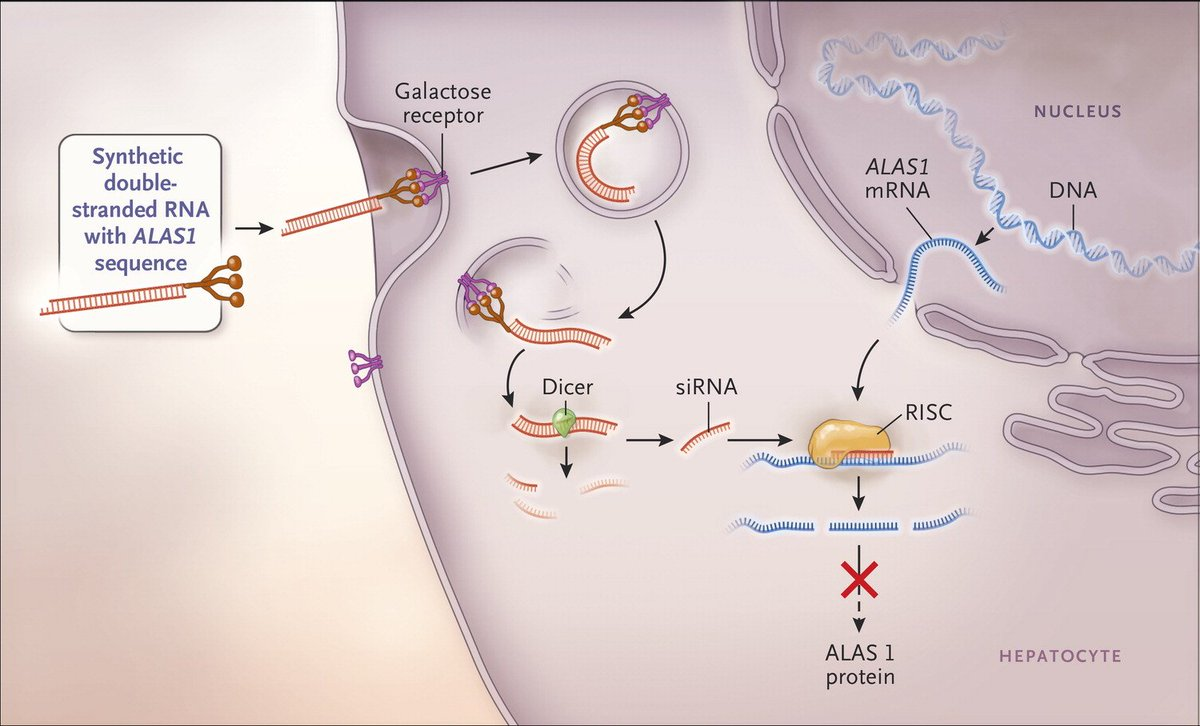
\includegraphics[width=\textwidth]{figures/pathophys-porphyria-therapy-sirna-nejm-original}
\caption[The Mechanism of Small Interfering RNA (siRNA) Therapy.]{\textbf{The Mechanism of Small Interfering RNA (siRNA) Therapy.} Synthetic double-stranded RNA containing an ALAS1-specific sequence is derivatized with N-acetylgalactosamine to target the asialoorosomucoid (galactose) receptor, which is expressed nearly exclusively on hepatocytes. Within the hepatocyte, the RNA is processed into approximately 20-bp fragments by a cellular enzyme (dicer), and then separated into single strands. The strand that is complementary to ALAS1 (the guide strand) binds to cellular ALAS1 messenger RNA (mRNA) and enters the RNA-induced silencing complex (RISC), where the new double-stranded RNA is cleaved by a group of factors that include argonaute, a ribonuclease. The result is a reduction in the level of delta ALA synthase 1 protein and decreased production of ALA. Image and caption by Dr. Gerald Diaz.\cite{Diaz2018}
\label{fig:pathophys-porphyria}}
\end{figure}

Another notable common characteristic of antisense therapeutics on the market or in the pipeline is the monogenetic or pseudo-monogenetic nature of the targeted diseases. For instance, in neurology, phase III pipeline candidates include IONIS-HTT$_{Rx}$ for treatment of Huntington's disease, and tofersen for treatment of SOD1-driven amyotrophic lateral sclerosis. Both diseases are characterised by a clear understanding of how changes in single transcripts cause pathology, and thus are easily accessible to the design of an antisense sequence. Inclisiran, also known as ALN-PCSsc, has recently successfully completed phase II trial for the treatment of familial hypercholesterinaemia.\cite{Raal2020} Its target is the \ac{pcsk} mRNA, reduction of which leads to a reduction in \ac{ldl} particles. Similarly to other liver-targeted oligonucleotides, inclisiran is hybridised to triantennary N-acetylgalactosamine carbohydrates, conveying liver-specific receptor-mediated endocytosis. The encapsulating lipid nanoparticles utilise the aminolipid DLin-MC3-DMA (see Figure \ref{fig:lipid}).\cite{Jayaraman2012} Inclisiran has been shown to significantly alleviate familial hyper"-chol"-es"-ter"-in"-aemia (\ac{ldl}-levels reduced by approximately 40\%) via only bi-annual subcutaneous application.\cite{Frank-Kamenetsky2008, Fitzgerald2014, Fitzgerald2017, Raal2020}

The use of single-target oligonucleotides parallels the dogma in modern medicinal chemistry of creating drugs with as little off-target effects as possible, to be able to tightly control the biological effects of the drug while simultaneously preventing adverse effects. Due to their extreme target specificity caused by mRNA complementarity, antisense oligonucleotides mainly cause adverse effects via their application (e.g., local effects at the subcutaneous injection site) or the compounds needed to facilitate their delivery (e.g., the lipid nanoparticles). Considering the very infrequent application as compared to other subcutaneous therapeutics, the general adverse effect risk of antisense therapy can be considered low.\cite{Raal2020}

The main problem in antisense therapy in its current state is the limitation to easily accessible compartments and the single-target nature of the drugs. All diseases featured in this dissertation (compare Section \ref{sec:intro:diseases} and Chapters 3 \& 4) are known for their polygenetic or poly-factorial nature, and thus, monogenetic therapeutic approaches are bound to fail. Additionally, psychiatric diseases present the major delivery hurdle of the blood-brain-barrier, and possibly pose advanced delivery problems such as single affected CNS cell types. Traditional small molecule therapeutics in psychiatric disease are known for their extreme range of target molecules. Most are derived from chlorpromazine, an artefact of antihistamine discovery synthesis, and are notorious for their targeting of multiple classes of neurotransmitter receptors. Impressively, second generation antipsychotics, which generally are seen as an improvement over the first generation of chlorpromazine-type antipsychotics, often present a more extensive and complex receptor profile, contrary to the specificity dogma of medicinal chemistry.

Translation of the knowledge of these dynamics in psychiatric diseases to antisense oligonucleotide therapy is the biggest hurdle for the design of adequate drug molecules. As opposed to small molecule drugs (high throughput screening of synthetic derivative molecules), serendipity is all but impossible in the case of antisense drugs, which are comprised of combinations of only four principal building blocks, as opposed to thousands of different chemical moieties, but a greater combinatorial multitude of possible molecules: $4^n$, with the common length of 22 nt, yields approximately 17.6 trillion individual molecules. The iterative screening of all possible combinations of the four bases in common high-throughput assays would quickly exceed experimental capacities and would lead to uneconomic development costs, particularly if seeking a multi-target oligonucleotide. Thus, bioinformatic predictions of suitable candidate molecules to be tested are necessary for efficient and economic screening of drug candidates for any given application, as well as for the prior identification of suitable combinations of target molecules in any given disease.

The dissertation here presented provides an infrastructure for these analysis steps (Chapter 2) as well as examples for high-prevalence diseases (Chapters 3 \& 4). Integrative transcriptomics analyses can serve as tools for the identification of pertinent pathways in pathogenesis as well as for the development of oligonucleotides with multi-target behaviour that enables synergistic effects in therapy and an imitation of multiple-target small molecule drug behaviour. Priorities in these analyses can be set to reflect the researchers' focus; for instance, an analytical prior could bias the search towards pharmacologically interesting targets that are so far inaccessible to small molecule drugs, such as IRF5 in inflammation (see Section \ref{sec:stroke:ffl-cd14}).\cite{Almuttaqi2019} Multi-target oligonucleotides can follow two principal design strategies: the mimicking or antagonising of extant endogenous smRNA molecules, such as miRNAs, or the de-novo creation of oligonucleotides based on complementarity to predefined target transcripts. The former method is more likely to be efficacious in a short time frame, but brings with it the risk of generating a plethora of adverse effects, because the target profiles of miRNAs are mostly very broad, tissue specific, and not entirely clear yet. De-novo design, on the other hand, theoretically allows the creation of defined target populations without off-target effects. The human genome is known, and thus, sequences can be generated that are complementary only to the target RNA molecules, without any other hits across the genome. However, since not all mechanistic aspects of RNA interference are clear (canonical versus non-canonical binding, bridging, wobble), not all complementary oligonucleotides are similarly effective. Thus, candidate molecules require thorough testing. This brings attention to another important limitation in de-novo design of oligonucleotide drugs: due to the differences in species genomes, these molecules cannot be comprehensively tested in animal models, particularly in rodents. Safety considerations thus should have utmost priority in clinical evaluation of such molecules. Studies of these phenomena have led to the new subfields of genocompatibility and toxicogenomics.\cite{Akhtar2007}

In immunology, hybridisation of oligonucleotide drugs to immune cell-specific receptor ligands could be used to convey a cell-type specificity akin to current liver-specific approaches. Many transcription factors show highly context-dependent activities,\cite{Hamada2020} and thus, a combination of TF specificity conveyed by the oligonucleotide and cell type specificity conveyed by a hybridisation partner may allow context-dependent intervention. For instance, ligands specific for CD4$^+$ cells could be used to target oligonucleotides to T helper cells, targeting relevant TFs such as NF-$\upkappa$B or STATs to modify the inflammatory reflex; oligonucleotides hybridised to CD14$^+$-targeting ligands could be utilised to interfere with monocyte responses, e.g. after stroke. Due to the trafficking of immune cells between brain and periphery, therapy of diseases with neuroinflammatory components could be accessible through the much easier peripheral (e.g., subcutaneous) application. Considering the accessibility of different tissues to standard parenteral application routes, the most promising strategies are targeting of immune cells circulating in the blood, or stationary in the spleen, both of which are relatively permissible to nanoparticles,\cite{Gullotti2009} and, in limited fashion, also lymph nodes, which can accommodate particle sizes between 10 and \SI{100}{\nano\metre}.\cite{Schudel2019} A knockdown of few select monocyte-specific transcripts could be used to drive differentiation towards the pro-resolving M2-type macrophage population,\cite{Panizzi2010} possibly breaking the vicious cycle of protracted inflammation. Co-targeting of cholinergic and neurokine transcripts may interfere more causally in pathogenesis of diseases with cholinergic participation than current single-target small molecule approaches.

%sexual differences